\documentclass{beamer}

\mode<presentation> {

% The Beamer class comes with a number of default slide themes
% which change the colors and layouts of slides. Below this is a list
% of all the themes, uncomment each in turn to see what they look like.

%\usetheme{default}
%\usetheme{AnnArbor}
%\usetheme{Antibes}
%\usetheme{Bergen}
%\usetheme{Berkeley}
%\usetheme{Berlin}
%\usetheme{Boadilla}
%\usetheme{CambridgeUS}
%\usetheme{Copenhagen}
%\usetheme{Darmstadt}
%\usetheme{Dresden}
%\usetheme{Frankfurt}
%\usetheme{Goettingen}
%\usetheme{Hannover}
%\usetheme{Ilmenau}
%\usetheme{JuanLesPins}
%\usetheme{Luebeck}
%\usetheme{Madrid}
%\usetheme{Malmoe}
%\usetheme{Marburg}
%\usetheme{Montpellier}
%\usetheme{PaloAlto}
%\usetheme{Pittsburgh}
%\usetheme{Rochester}
\usetheme{Singapore}
%\usetheme{Szeged}
%\usetheme{Warsaw}
\setbeamertemplate{footline}[frame number]

% As well as themes, the Beamer class has a number of color themes
% for any slide theme. Uncomment each of these in turn to see how it
% changes the colors of your current slide theme.

%\usecolortheme{albatross}
%\usecolortheme{beaver}
%\usecolortheme{beetle}
%\usecolortheme{crane}
%\usecolortheme{dolphin}
%\usecolortheme{dove}
%\usecolortheme{fly}
%\usecolortheme{lily}
%\usecolortheme{orchid}
%\usecolortheme{rose}
%\usecolortheme{seagull}
%\usecolortheme{seahorse}
%\usecolortheme{whale}
%\usecolortheme{wolverine}


}

\usepackage{graphicx} 
\usepackage{booktabs} 
\usepackage{hyperref}
\usepackage{amssymb}
\usepackage{mathtools}
\usepackage{amsthm}
\usepackage{tikz-cd}
\usepackage{array}
\usepackage{yfonts}
\usepackage{soul}

\theoremstyle{mystyle}
\newtheorem*{conjecture}{Conjecture}
\newtheorem*{principle}{Principle}

\newcommand {\bra} [1] {\ensuremath{ \left\langle #1 \right| }}
\newcommand {\ket} [1] {\ensuremath{ \left| #1 \right\rangle }}
\newcommand {\ketbratwo} [2] {\ensuremath{ \left| #1 \middle\rangle \middle\langle #2 \right| }}
\newcommand {\ketbra} [1] {\ketbratwo{#1}{#1}}
\newcommand {\suppress} [1] {}
\newcommand {\eps} {\varepsilon}
\newcommand {\dmax} [2] {\ensuremath{\mathrm{D}_{\max}(#1 \| #2)}}
\newcommand {\relent} [2] {\ensuremath{\mathrm{D}(#1 \| #2)}}
\newcommand {\id} {\mathrm{I}}
\newcommand {\Tr}{\mathrm{Tr}}
\newcommand {\bluu}[1]{\textcolor{blue}{#1}}
\newcommand {\br}[1]{\left(#1\right)}
\newcommand {\cA}{\mathcal{A}}
\newcommand {\cH}{\mathcal{H}}

\newcommand {\beit}{\begin{itemize}}
\newcommand {\enit}{\end{itemize}}

\newcommand{\frmt}[1]{\frametitle{#1}}

\title[QSE 210A/Phys 260A: Lecture 0]{Lecture 0: Introduction} 

\author{Anurag Anshu} 

%\AtBeginSection[]
%{
 % \begin{frame}<beamer>
  %  \frametitle{Upcoming section}
  %  \tableofcontents[currentsection]
 % \end{frame}
%}

\begin{document}


\begin{frame}
\titlepage 
\end{frame}

\begin{frame}{Rapid developments in quantum computing}

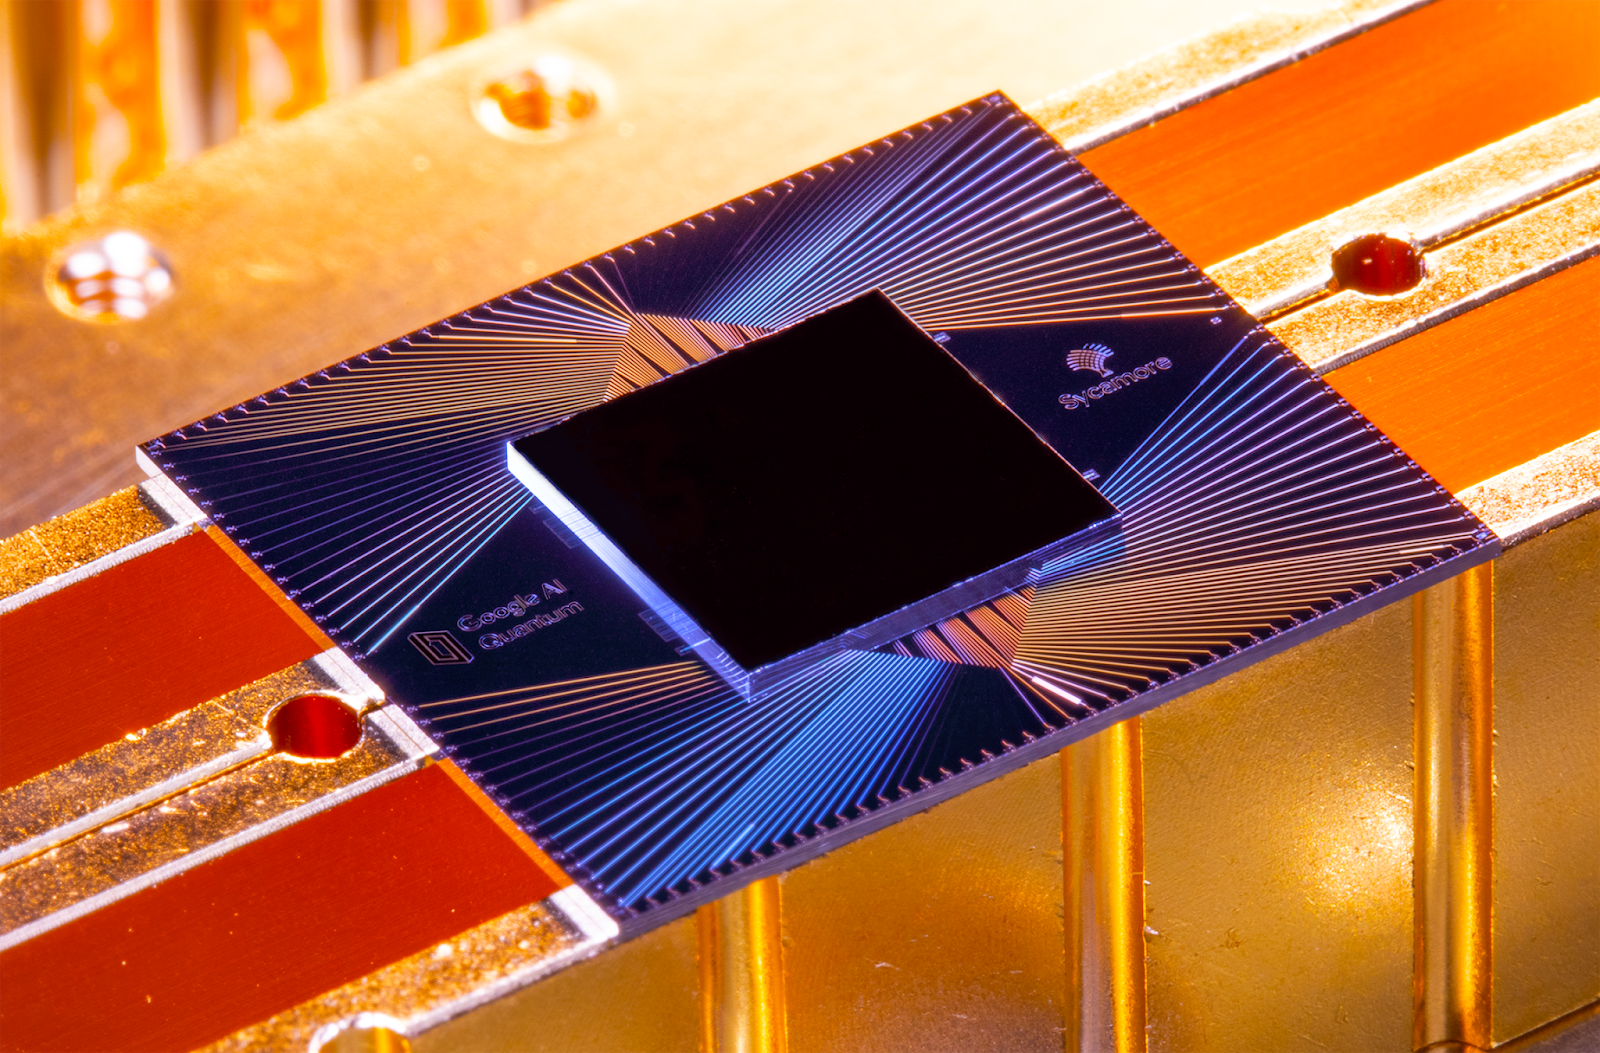
\includegraphics[scale=0.08]{Lecture notes/Lec 0 Presentation/sycamore.png}
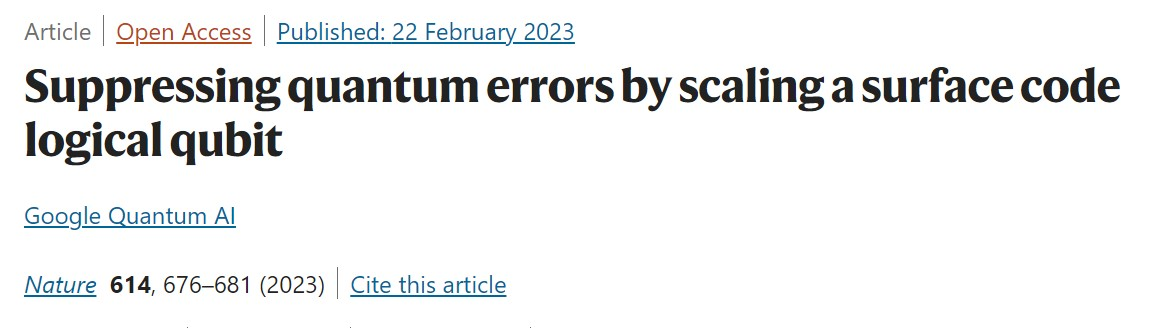
\includegraphics[scale=0.3]{Lecture notes/Lec 0 Presentation/googlelogical.jpg}

\vspace{0.1in}

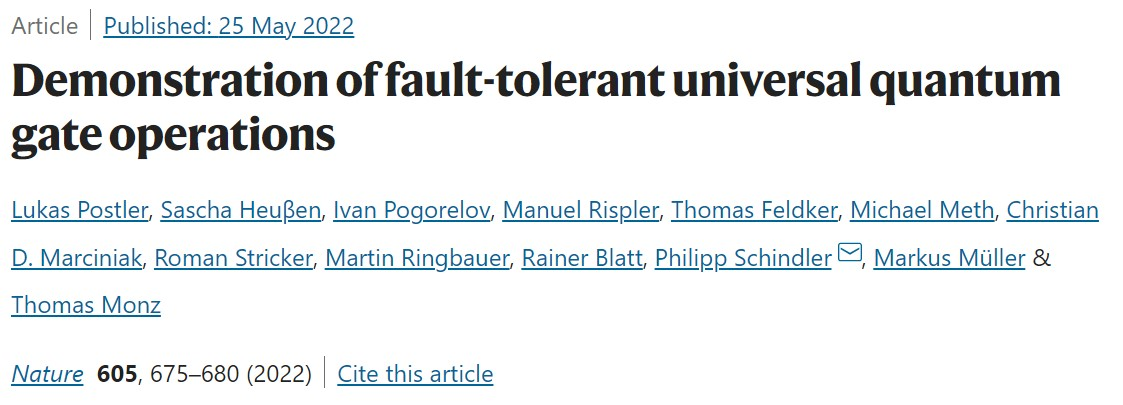
\includegraphics[scale=0.25]{Lecture notes/Lec 0 Presentation/FT.jpg}
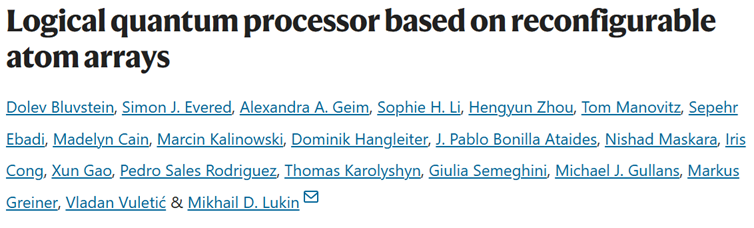
\includegraphics[scale=0.4]{Lecture notes/Lec 0 Presentation/Logicalproc.png}
    
\end{frame}

\begin{frame}{Quantum hype?}

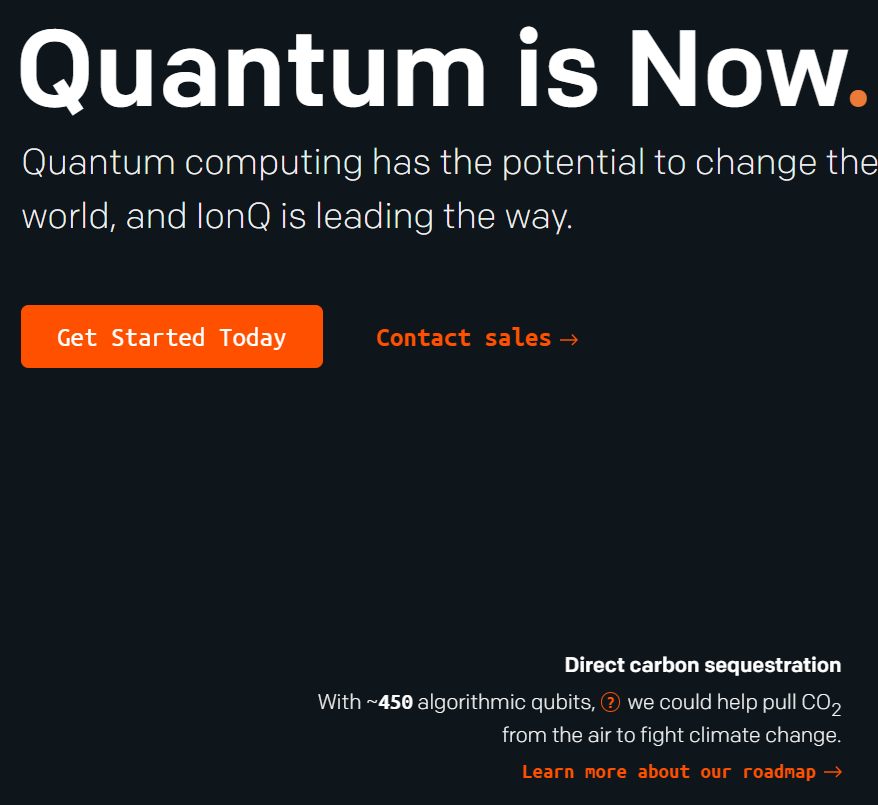
\includegraphics[scale=0.3]{Lecture notes/Lec 0 Presentation/Qhype.png}
\pause
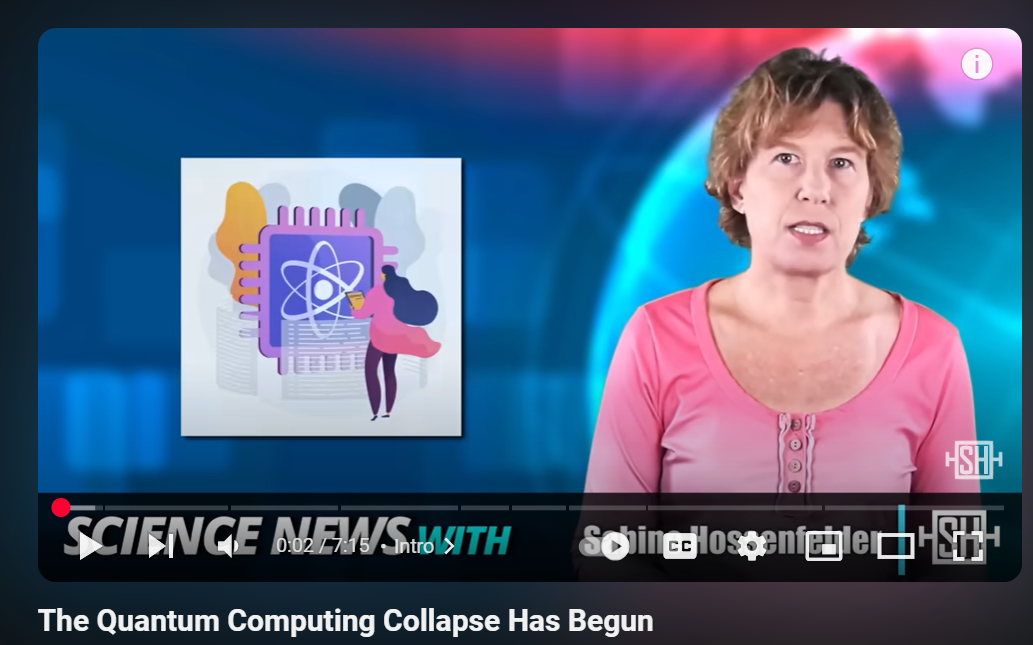
\includegraphics[scale=0.3]{Lecture notes/Lec 0 Presentation/Collapse.png}

\pause

\vspace{0.1in}

Hype or anti-hype based on the limiting view that quantum computing is all about delivering practical (and possibly commercial) computational advantage.
    
\end{frame}

\begin{frame}{Remarkable achievements of quantum computing/quantum information}

\begin{itemize}
    \item Discovery of new physical phenomena from quantum simulators
\end{itemize}

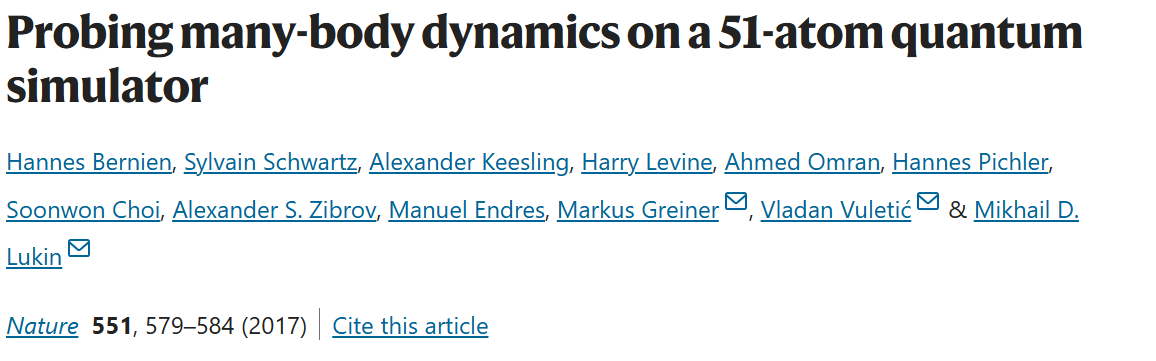
\includegraphics[scale=0.5]{Lecture notes/Lec 0 Presentation/Scarnature.png}
    
\end{frame}

\begin{frame}{Remarkable achievements of quantum computing/quantum information}

\begin{itemize}
    \item Resolution of 50-year-old open problem in mathematics.
\end{itemize}

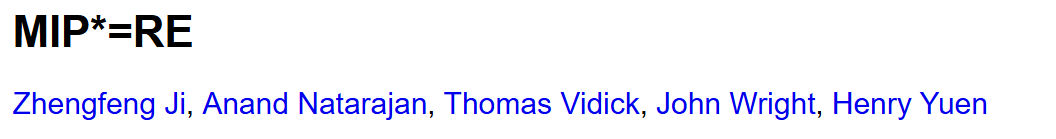
\includegraphics[scale=0.5]{Lecture notes/Lec 0 Presentation/MIPstar.png}
    
\end{frame}

\begin{frame}{Remarkable achievements of quantum computing/quantum information}

\begin{itemize}
    \item First rigorous proof of half-century old physics heuristics
\end{itemize}

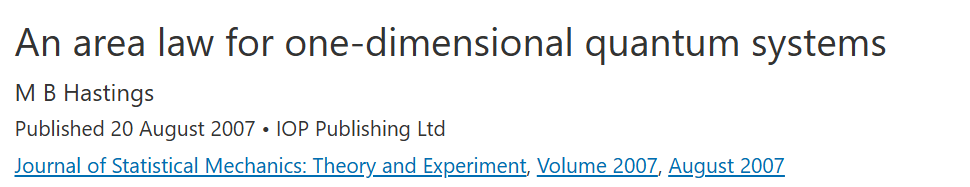
\includegraphics[scale=0.5]{Lecture notes/Lec 0 Presentation/hastings.png}

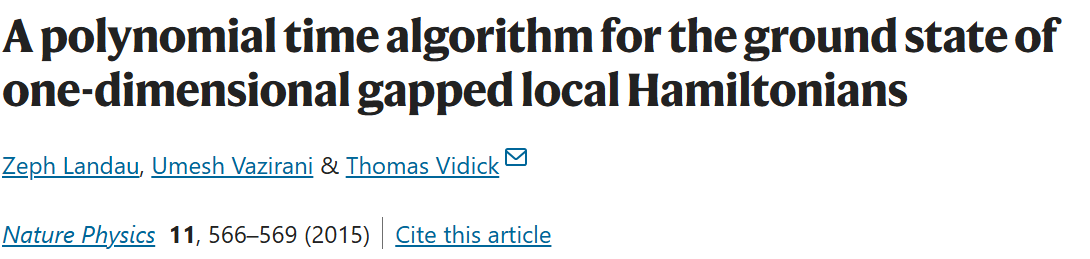
\includegraphics[scale=0.5]{Lecture notes/Lec 0 Presentation/AGSP.png}


    
\end{frame}

\begin{frame}{Remarkable achievements of quantum computing/quantum information}

\begin{itemize}
    \item New theoretical phases of matter
\end{itemize}

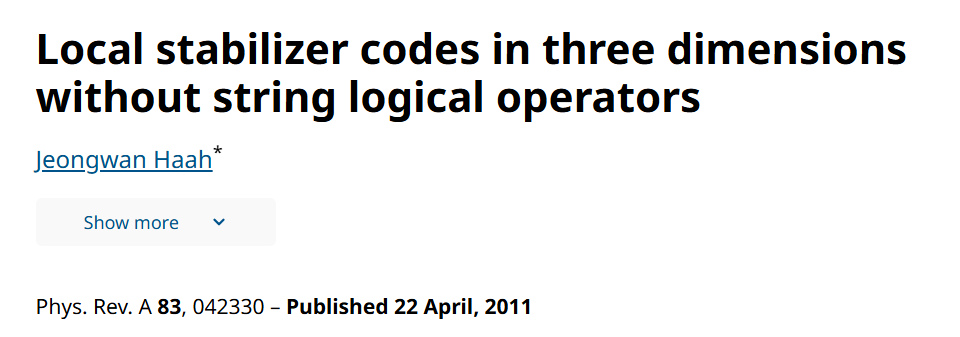
\includegraphics[scale=0.5]{Lecture notes/Lec 0 Presentation/haah.png}
    
\end{frame}

\begin{frame}{Important themes: Quantum algorithms}

\begin{itemize}
    \item Quantum advantage in quantum algorithms and non-locality.
    \item Non-local games, Grover's search and Shor's algorithm. 
    \item Why quantum algorithms solve some problems fast and do not solve other problems fast?
\end{itemize}


    
\end{frame}


\begin{frame}{Important themes: Quantum fault tolerance}

\begin{itemize}
    \item Fighting noise in quantum computation.
    \beit
    \pause
    \item Quantum mechanics feels continuous, but it is actually discrete.
    \pause
    \item Discrete view of quantum mechanics crucial in quantum fault tolerance theorems.
    \enit
\end{itemize}

\pause

\vspace{0.1in}

\centering

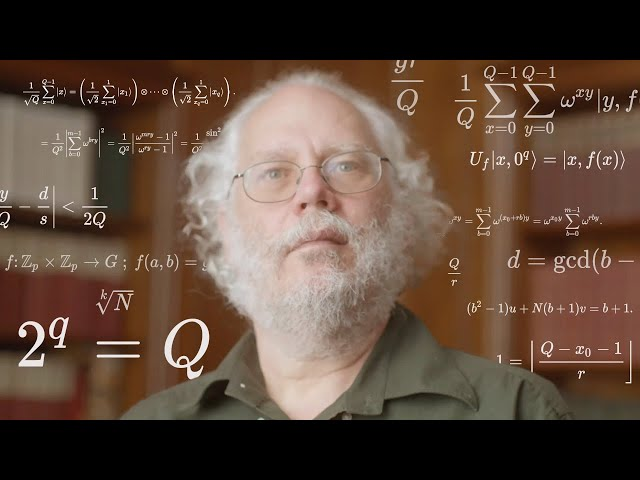
\includegraphics[scale=0.15]{Lecture notes/Lec 0 Presentation/shor.jpg}
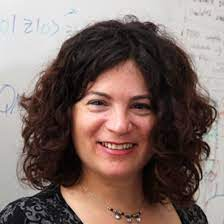
\includegraphics[scale=0.33]{Lecture notes/Lec 0 Presentation/aharonov.jpeg}
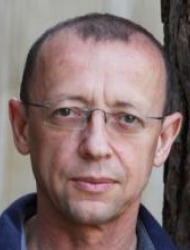
\includegraphics[scale=0.4]{Lecture notes/Lec 0 Presentation/benor.jpg}
    
\end{frame}

\begin{frame}{Important themes: Quantum computing and physics}

\begin{itemize}
    \item Quantum algorithms lead to most efficient (theoretically speaking) ways to simulate physical systems.
\end{itemize}


\begin{tikzpicture}[xscale=0.3,yscale=0.3]
	\node at (0,0) {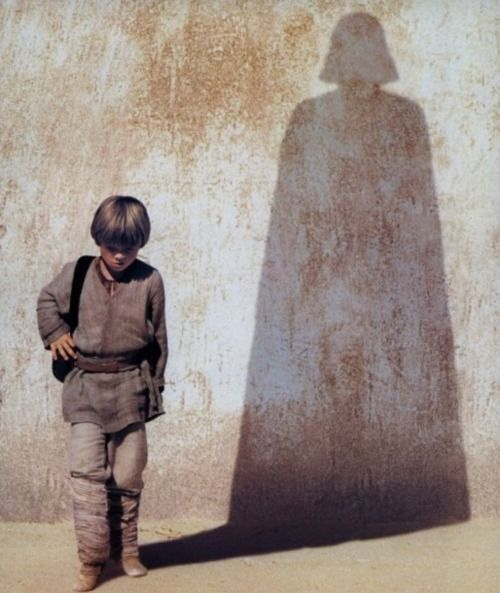
\includegraphics[scale=0.2]{Lecture notes/Lec 0 Presentation/anakin.jpg}};
	\node at (-10,0) {\textcolor{blue}{\small Grover's search}};
%	\node at (5,2) {\textcolor{blue}{Quantum walks}};
%	\node at (5,1) {\textcolor{blue}{Quantum signal processing}};
%	\node at (5,0) {\textcolor{blue}{Gibbs state preparation}};
	\node at (10,0) {\textcolor{blue}{Hamiltonian simulation}};
    \end{tikzpicture}

\pause

\begin{itemize}
    \item Quantum computing explains why several physics problems, like estimating ground energy, are hard.
\end{itemize}
    
\end{frame}

\begin{frame}
\frmt{Course components beyond lectures}
\beit
\item Sender-receiver exercises: various important concepts discussed through in-class activities. Three days before the exercise:
\pause
\beit
\item Senders will be given a handout with a statement and proof of an important theorem.
\item Receivers will be given the statement of the theorem.
\item Senders will be paired up with receivers in class and they will explain the theorem to the receivers. 
\enit
\pause
\item Final projects (in groups of 2-3): various possible project topics will be suggested mid-semester.  
\beit
\item Report to be submitted by the end of the semester. 
\item Final presentations (at least one member per group must be present).
\enit
\enit
\end{frame}


\begin{frame}
\frmt{Quantum theory}
\centering

\includegraphics[scale=0.35]{Lecture notes/Lec 0 Presentation/joke.png}
\end{frame}

\end{document} 